\newpage
\begin{center}
	\textbf{\large 2. МОДЕЛИ ВРЕМЕННЫХ РЯДОВ}
\end{center}
\refstepcounter{chapter}
\addcontentsline{toc}{chapter}{2. МОДЕЛИ ВРЕМЕННЫХ РЯДОВ}

В этой главе будут рассмотрены некоторые модели временных рядов
с помощью которых можно решать задачу прогнозирования ожидаемой доходности активов.
Проверка на реальных данных качества прогнозирования и доходностей портфелей, 
построенных с импользованием рассматриваемых моделей, будет приведена в главе 3.


\section{Общий подход к прогнозированию рядов}

Процесс прогнозирования заключается в оценке будущего значения временного ряда либо путем 
моделирования ряда исключительно на основе его прошлого поведения (авторегрессия), либо путем включения других внешних переменных.

Чтобы применить модели машинного обучения к задачам прогнозирования, временной ряд необходимо преобразовать в матрицу, 
где каждое значение связано с определенным прерыдущим значением ряда (лагом). 
В контексте временного ряда, лаг относительно момента времени $t$ определяется как значение ряда на предыдущих временных шагах. 
Например, лаг $1$ представляет значение на временном шаге $t-1$, тогда как лаг $m$ представляет значение на временном шаге $t-m$. 

Это преобразование необходимо для моделей машинного обучения для захвата зависимостей и закономерностей, которые существуют 
между прошлыми и будущими значениями во временном ряду. Используя лаги в качестве входных признаков, модели машинного 
обучения могут учиться на прошлом и делать прогнозы относительно будущих значений. Количество лагов, используемых в качестве 
входных признаков в матрице, является важным гиперпараметром, который необходимо тщательно настраивать для получения наилучшей 
производительности модели.

Модели машинного обучения в основном заточены на решение табличных задач. Однако, они несложным образом адаптируются 
для пронозирования временных рядов.
Признаки формируются как лаги временного ряда. Процесс формирования матрицы объекты-признаки схематично
показан на рисунке \ref{fig:feature_matrix}.

\begin{figure}[H]
	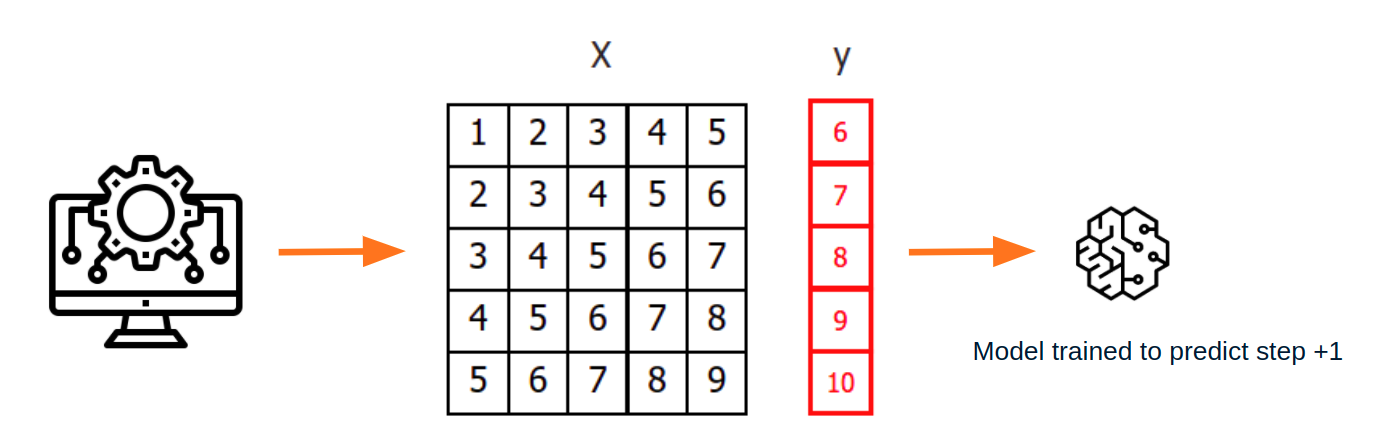
\includegraphics[width=\textwidth]{ts_xy}
	\caption{Матрица объекты-признаки}
	\label{fig:feature_matrix}
\end{figure}

После того, как данные были перестроены в новую форму, любая регрессионная модель может быть обучена прогнозировать 
следующее значение (шаг) ряда. Во время обучения модели каждая строка считается отдельным экземпляром данных, 
где значения на лагах $1, 2, \dots p$ считаются предикторами для целевого количества временного ряда на временном шаге $p+1$.

\begin{figure}[H]
	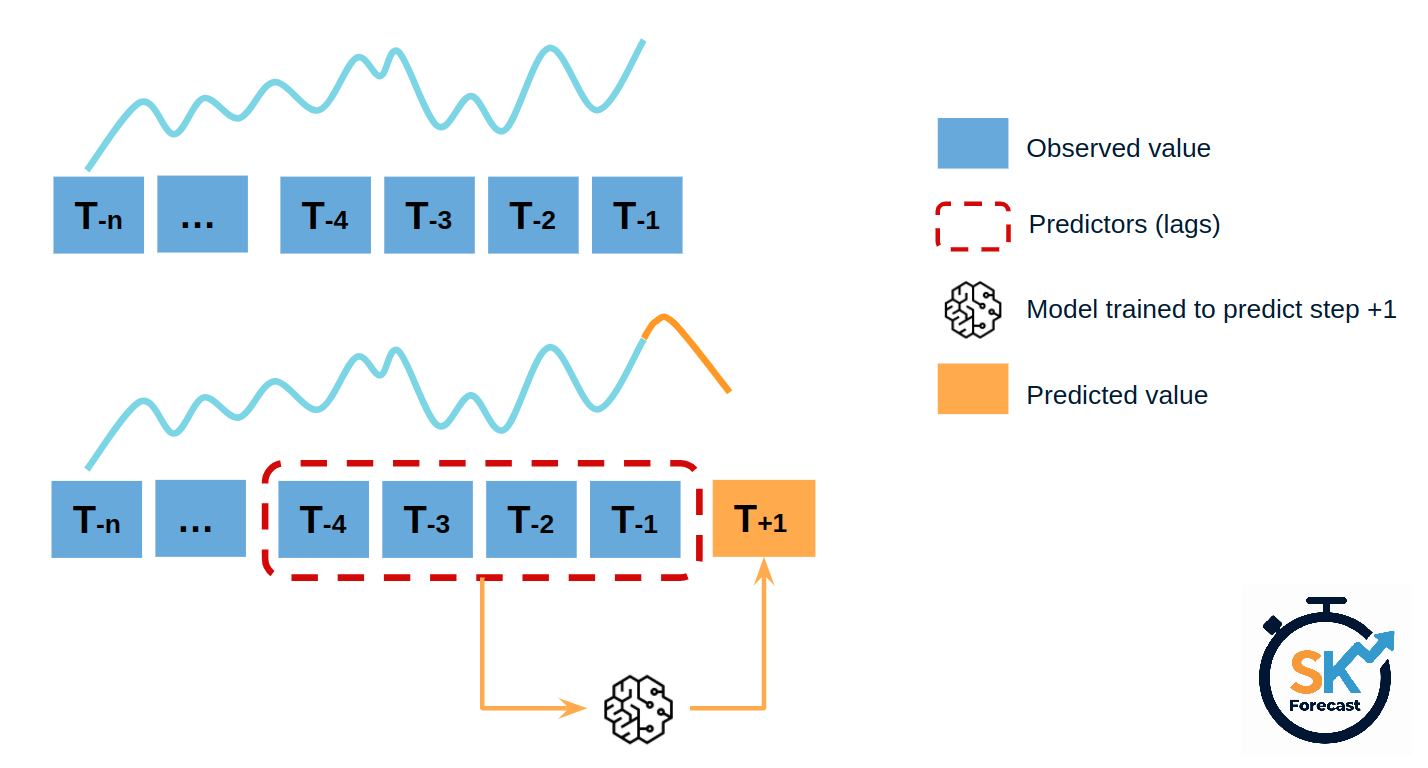
\includegraphics[width=\textwidth]{ts_predictors}
	\caption{Формирование признаков как временных лагов ряда}
\end{figure}

В прогнозировании временных рядов процесс бэктестинга заключается в оценке производительности предсказательной модели путем ее 
ретроспективного применения к историческим данным. Таким образом, это особый тип перекрестной проверки, применяемый к предыдущим
периодам.

Цель бэктестинга --- оценить точность и эффективность модели . 
Проверяя модель на исторических данных, можно оценить насколько хорошо она работает на данных, которые она ранее не видела. 
Это важный шаг в процессе моделирования, поскольку он помогает гарантировать, что модель является надежной и устойчивой.

Бэктестинг можно проводить с использованием различных методов, таких как простые разделения обучения и тестирования или более 
сложные методы, такие как скользящие окна или расширяющиеся окна. Выбор метода зависит от конкретных потребностей анализа и 
характеристик данных временных рядов.

\begin{figure}[H]
	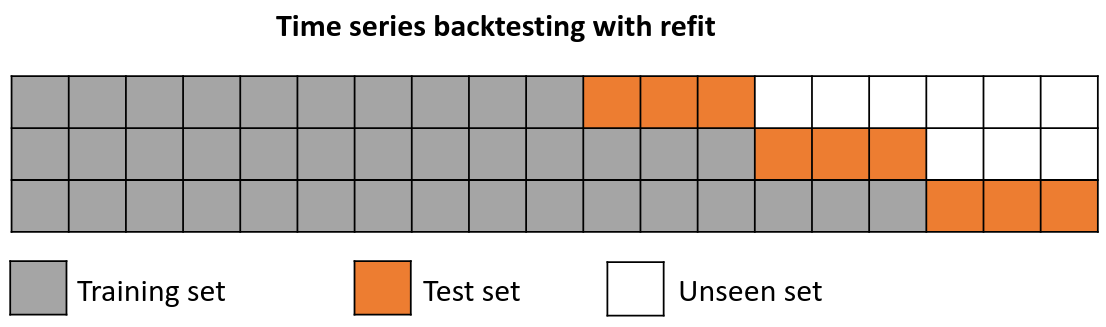
\includegraphics[width=\textwidth]{ts_backtest}
	\caption{Формирование выборок при бектестинге}
\end{figure}

Будем использовать подход с расширением обучающего множества и переобучением на каждом шаге.
При таком подходе модель обучается перед каждым прогнозированием, и все доступные данные на тот момент используются в процессе обучения. 
Это отличается от стандартной перекрестной проверки, где данные случайным образом распределяются между обучающими и проверочными наборами.

Вместо рандомизации данных этот бэктестинг последовательно увеличивает размер обучающего набора, сохраняя временной порядок данных. 
Благодаря этому модель можно тестировать на все больших объемах исторических данных, что обеспечивает более точную оценку ее 
качества прогнозирования.

\section{Линейная регрессия} 
\label{sec:LR}

Пусть $X$ и $Y$ матрица обектов-признаков и вектор целевых значений, построенные по историческим данным.

Линейная регрессия есть линейная комбинация признаков (лагов) $x$ и весов $w$.
\begin{align}
	a(x) = w_0 + w_1 x_1 + \dots + w_n x_n = \left< x, w \right>
\end{align}

Решение $w^*$ находится методом наименьших квадратов. 
Определим функционал потель как средний квадрат ошибки модели на всех элементах выборки.
\begin{align}
	Q(a) = \frac{1}{\ell} \sum_{i=1}^{\ell} \left( y_i - a(x_i)\right)^2 = ||Xw - y||^2
\end{align}

Необходимое условие минимума
\begin{align}
	\frac{\partial Q}{ \partial w} = 2X^T(Xw - y) = 0
\end{align}

Решая систему уравнений получим аналитический вид решения оптимизационной задачи
\begin{align}
	w^* = \left(X^TX\right)^{-1}X^Ty
\end{align}

Огромным преимуществом данной модели является её простота и скорость обучения. Также веса модели можно интерпретировать.
Большие абслолютные значения весов означают сильный вклад соответсвующих лагов в целевую переменную. Далее перейдем к
рассмотрению более сложных моделей.


\section{Случайный лес}
\label{sec:RF}

Алгоритм случайного леса есть простое голосование над решающими деревьями. Он является одним из сильнейших алгоритмов машинного обучения.
Описывается основная идея работы алгоритма, а более подробно об этом алгоритме написано в статье \cite{random_forest}.

Дерево решений есть бинарное дерво. Определены вершины двух типов: 
\begin{itemize}
	\item внутренние --- содержит предикат $b_v : \mathbb{X}\rightarrow \{0, 1\}$
	\item листовые --- хранит выходное значение $c_v \in \mathbb{Y}$
\end{itemize}

Этапы обработки деревом входящего объекта $x$
\begin{enumerate}
	\item Стартуем из корня
	\item Вычисляем текущий предикат $b_v(x)$
	\item Если $b_v(x) = 0$ то делаем шаг в левое поддерево, иначе --- в правое
	\item Пока не дошли до листовой вершины, повторяем шаги 2 и 3
	\item Возвращаем значение $c_v$ в листе
\end{enumerate}

В качестве базовых алгоритмов выберем набор решающих деревьев $b_1, \dots, b_k$.
Объеденим результаты работы базовых алгоритмов с помощью простого голосования
\begin{align}
	a(x) = \frac{1}{k} \sum_{i=1}^{k} b_i(x)
\end{align}

Ошибку работы ансамбля можно разложить на 3 компоненты
\begin{align}
	Q(a) = bias(a) + variance(a) + noiсe
\end{align}
где
\begin{align}
	bias(a) = f(x) - \mathbb{E}_X\left[a(x, X)\right] \\
\end{align} 
--- смещение алгоритма,
\begin{align}
	variance(a) = \mathbb{E}_X\left[a(x, X)\right] -\mathbb{E}_X\left[a(x, X)\right]^2 \\
\end{align}
--- разброс алгоритма,
\begin{align}
	noiсe = \mathbb{E}_X\left[\mathbb{E}_{\epsilon}\left[\left( y(x, \epsilon) - f(x) \right)^2\right]\right]
\end{align}
--- неустранимый шум.

Смещение ансамбля определяется смещением базового алгоритма. Поэтому разумно строить неглубокие деревья.
\begin{align}
	bias(a) = 
	f(x) - \mathbb{E}_X\left[a(x, X)\right] = \\
	= f(x) - \mathbb{E}_X\left[\frac{1}{k} \sum_{i=1}^{k} b(x, X^i)\right] = \\
	= f(x) - \mathbb{E}_X\left[b(x, X)\right] = \\
	= bias_X(b)
\end{align}

Разброс ансамбля определяется числом базовых алгоритмов в нем и корреляциями между ними.
Постараемся добиться некоррелированности, или, по крайней мере, непохожести базовых алгоритмов за счет обучения
каждого из нах на разных данных. С этим помогает идея бутстрапирования.

\begin{align}
	variance(a) & = \mathbb{E}_X\left[a(x, X) - \mathbb{E}_x\left[a(x, X)\right]\right]^2 = \\
	& = \mathbb{E}_X\left[\frac{1}{k} \sum_{i=1}^{k} b_i - \mathbb{E}_X\left[\frac{1}{k} \sum_{i=1}^{k}\right]\right]^2 = \\
	& = \frac{1}{k^2} \mathbb{E}_X\left[\sum_{i=1}^{k} \left( b_i - \mathbb{E}_X\left[b_i \right]\right)\right]^2 = \\
	& = \frac{1}{k^2} \sum_{i=1}^{k} variance_X(b_i) + 
	\frac{1}{k^2} \sum_{i \ne j} \COV{b_i}{b_j}
\end{align}

Помимо алгоритмов машинного обучения для прогнозирования временных рядом можно воспользоваться классическими моделями временных рядов.
Одной из них является модель ARIMA.

\section{ARIMA}
\label{sec:ARIMA}

Модель ARIMA обобщает модель ARMA. Подробно работа модели описывается здесь \cite{shiryaev_finmat_1}.

Модель $ARMA(p, q)$ сочетает в себе моедли авторегрессии $AR(p)$ и скользящего среднего $MA(q)$.

Пусть задано фильтрованное вероятностное пространство $\left( \Omega, \mathscr{F}, (\mathscr{F}_n), P \right)$
Будем считать что $\mathscr{F}_n = \sigma(\dots, \epsilon_{-1}, \epsilon_0, \epsilon_1, \dots, \epsilon_n)$ с белым шумом $\epsilon = (\epsilon_n)$.

По определению, последовательность $x = (x_n)$ является ARMA-моделью, если 
\begin{align}
	x_n = \mu_n + \sigma \epsilon_n
\end{align}
где
\begin{align}
	\mu_n = \left(a_0 + a_1 x_{n-1} + \dots + a_p h_{n-p} \right) +
	\left(b_1 \epsilon_{n-1} + b_2 \epsilon_{n-2} + \dots + b_q \epsilon{n - q} \right)
\end{align}

Эта модель допускает обобщение на случай когда исходный ряд не стационарен. А именно, расммотрим разности процесса $x$
\begin{align}
	\Delta x_n = x_n - x_{n-1}
\end{align}

Повторяя операцию взятия разности $d$ раз, получим процесс $\Delta^d x = (\Delta^d x_n)$. Если полученный процесс <<более стационарный>>
чем исходный, то построим уже для него $ARMA(p, q)$ модель.

Описанная модель есть трехпараметрическая модель временного ряда $ARIMA(p, d, q)$. Символически это можно записать
\begin{align}
	\Delta^d ARIMA(p, d, q) = ARMA(p, q)
\end{align}

В этой главе были рассмотрены некоторые алгоритмы построения моделей временных рядов позволяющие строить прогноз будущих значений на основании
истории ряда. Применение эти модели для оценки будущих средних доходностей в теории Марковица, позволяет строить множества оптимальных портфелей.
Перейдем к построению и оценке инвесиционных стратегий, основанных на рассмотренных моделях.